% Drawing 154/06-22 -- folder 154, batch 06, archive page 104 (PDF page 105).
% Transcription: la moitié inférieure de la page est faite de dessins en couleur : deux paires de droites orange coupées par une droite vert clair, les sommets $x$, $y$, $z'$, $y'$ reliés par des chemins en tirets vert foncé ; le même avec des points $z$, $t$ et un chemin en tirets ; deux rectangles bordés de vert clair d'où partent des rayons en étoile, les côtés marqués $\alpha$, $\beta$, $\gamma$ et les coins $x$, $y$, $x'$, $y'$, étiquetés $(1)$, $(2)$, $(3)$, $(4)$, entourés de petits carrés vert clair ; un petit carré vert clair avec des flèches $\lambda$, $\mu$ entre $x$, $y$, $x'$ ; un faisceau de droites orange presque parallèles, la droite verte passant par-dessus ; enfin, une droite vert foncé coupée de droites orange, avec les légendes $\nu - 2$, $2$, $2$
% Kind: page of small figures: dashed paths, rayed rectangles, sheaves. Method 2 (schematic redraw from the facsimile). Status: partial.
% Notes: Eight figures, placed as on the page. Top left: two crossings z', y' above the light green line, the dark green dashed paths z'y', z'y, y'x and xy. Top middle: crossings z and t, the dashed path from z down to the line, along it and up to t, and the dashed piece of the line from x to y. Top right: the light green line making a tall bump over a sheaf of nearly parallel orange strokes between two crossings, short red strokes below (redrawn on 14 November, see below). Middle left: a rectangle with eight dashed rays from its centre, a dark green stroke from each corner to a small light green square; the pencil hatching, the Greek letters around it and the orange strokes along the corner segments are left out. Middle: the rectangle with a star of twenty orange arrows from its centre to its sides, the letters gamma, beta, alpha on three sides and beta on the fourth, the corners y', x', x, y, the numbers (2), (1) (the (3) above belongs to the second figure). Below: the small square with three arrows, lambda, mu, x', x, y; a sheaf of three strokes between two crossings; the dark green line with a crossing at each end, four barred orange strokes across it, a pencil arc, nu - 2 with its arrow, 2 and 2, and a brace below read nu. Positions as read; the figure is a simplification of a dense page. Redrawn 2026-11-12 (issue 128): to check again. 2026-11-14, Claude Opus 5.5, overlay check (issue 147): rasterised from its own coordinates over the 400 dpi colour scan (402 ppi native) on a unit grid; not compiled (no TeX in the session). Changed: the top right figure lay 1 to 3 units off its ink (a sheaf of five vertical strokes, a green bump too wide) and is redrawn on a 40 px per unit crop: the two crossings, the left leg of the left crossing and the right leg of the right one bent at the top into the shoulders of the arch; three orange strokes (not five) running down from a zigzag orange crown that joins their tops; the light green line solid up the left shoulder, in three dashes across the top and solid down the right shoulder to the right crossing; four short dark red strokes below (two crossing at the left, two meeting in a V). Laid over the scan again, it lies on its ink to within about 0.5 unit. The other seven figures lie on their ink to within about 1 unit (the small squares of the middle left figure, tilted on the page, are drawn upright). Still differs, hence partial: the pencil hatching, the Greek letters and the orange strokes round the middle left rectangle, the row of small pencil ticks above the dark green line and the small light green loops at its two ends are not drawn.
% Coordinates: 1 unit = 1 mm = 1/100 of the crop width (bbox in page fractions: [0.12, 0.325, 0.88, 0.54]).
% Redrawn by Claude (claude-fable-5-2), issue #128, 2026-11-12; not checked by a human; not compiled (no TeX in the session).
% Checked by Claude (claude-opus-5-5) 2026-11-14 (issue #147): overlaid on the 400 dpi colour facsimile; not compiled (no TeX in the session). Not checked by a human. Status: partial.
% Rights: reproduces part of the work -- behind RENDER_TRANSCRIPTS, never published by itself.
\documentclass[tikz,border=3pt]{standalone}
\usepackage{amsmath,amssymb}
\usetikzlibrary{patterns,arrows.meta}
\tikzset{Or/.style={orange!90!black}, Lg/.style={green!60!black!70}, Dg/.style={green!45!black}, Rd/.style={red!85!black}, pencil/.style={black!45}, struck/.style={black!35}, mpt/.style={circle,draw,inner sep=1.3pt}, pt/.style={circle,fill,inner sep=0.9pt}, opt/.style={circle,draw,fill=white,inner sep=1.1pt}}
\begin{document}
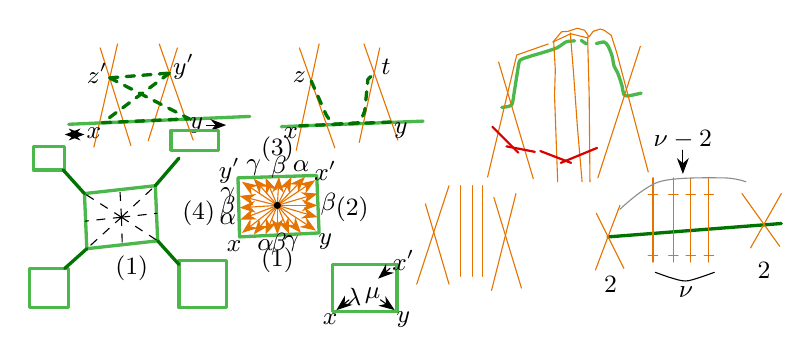
\begin{tikzpicture}[x=1mm,y=1mm,line cap=round,line join=round,font=\scriptsize]
\draw[Lg,very thick] (7,-13.7) -- (30,-12.7);
\draw[Or] (11,-4) -- (14.9,-16.4);
\draw[Or] (13.2,-3.5) -- (10.2,-16.6);
\draw[Or] (18.5,-3.5) -- (22.8,-15.7);
\draw[Or] (20.8,-4) -- (17.1,-15.8);
\draw[Dg,dashed,very thick] (12.2,-7.8) -- (19.8,-7.2);
\draw[Dg,dashed,very thick] (12.2,-7.8) -- (22.3,-13);
\draw[Dg,dashed,very thick] (19.8,-7.2) -- (11.3,-13.5);
\draw[Dg,dashed,very thick] (11.3,-13.5) -- (22.3,-13);
\node[inner sep=1pt] at (10.6,-7.2) {\small $z'$};
\node[inner sep=1pt] at (21.6,-6.4) {\small $y'$};
\node[inner sep=1pt] at (10.2,-14.8) {\small $x$};
\node[inner sep=1pt] at (23.2,-13.8) {\small $y$};
\draw[-{Stealth[length=2mm]}] (24.5,-13.8) -- (27,-13.8);
\draw[{Stealth[length=2mm]}-{Stealth[length=2mm]}] (6.5,-15) -- (9,-15);
\draw[Lg,very thick] (34,-14) -- (52,-13.3);
\draw[Or] (36.3,-4) -- (40.8,-16.7);
\draw[Or] (38.8,-3.5) -- (35.9,-17);
\draw[Or] (44.5,-3.5) -- (48.8,-15.7);
\draw[Or] (46.5,-4) -- (43.9,-16);
\draw[Dg,dashed,very thick] (37.8,-8.2) -- (39.7,-12.5) -- (40.5,-13.7) -- (44,-13.5) -- (44.6,-12) -- (45,-8) -- (45.8,-7.2);
\draw[Dg,dashed,very thick] (36.3,-13.9) -- (48.2,-13.4);
\node[inner sep=1pt] at (36.3,-7.7) {\small $z$};
\node[inner sep=1pt] at (47.3,-6.4) {\small $t$};
\node[inner sep=1pt] at (35.2,-14.8) {\small $x$};
\node[inner sep=1pt] at (49.2,-14.5) {\small $y$};
\node[inner sep=1pt] at (33.5,-16.9) {\small (3)};
\draw[Lg,very thick] plot[smooth, tension=0.4] coordinates {(62,-11.55) (63.25,-11.25) (63.6,-9.5) (64,-7) (64.3,-5.6) (65.5,-5.1) (67.5,-4.5) (69,-4) (69.75,-3.5) (70.25,-3.2) (71.25,-3.1)};
\draw[Lg,very thick] (72.1,-3.05) -- (72.75,-3.5);
\draw[Lg,very thick] plot[smooth, tension=0.4] coordinates {(74,-3.45) (75,-3.25) (75.5,-3.75) (76,-5) (76.25,-6.25) (76.75,-7.25) (77.25,-8.75) (77.5,-9.9) (78,-10.1) (79.7,-9.75)};
\draw[Or] (61.6,-5.8) -- (66,-20.6);
\draw[Or] (60.2,-20.4) -- (63.9,-4.9) -- (67.9,-3.5);
\draw[Or] (80.6,-19.75) -- (76.6,-4.6) -- (75.9,-2.4);
\draw[Or] (79.6,-3.8) -- (74.2,-20.5);
\draw[Or] (68.5,-3.25) -- (69.6,-1.95) -- (70.4,-1.9) -- (71.6,-1.5) -- (72.5,-1.75) -- (73.1,-2.6) -- (73.6,-1.9) -- (74.5,-1.6) -- (75,-1.75) -- (75.9,-2.4);
\draw[Or] (68.5,-3.25) -- (70.75,-2.2) -- (73,-2.75);
\draw[Or] (68.6,-3.3) -- (68.8,-6.8) -- (68.7,-10) -- (69.1,-21);
\draw[Or] (70.7,-2.1) -- (71.1,-7) -- (71.6,-14) -- (72.2,-21);
\draw[Or] (72.9,-2.6) -- (73.1,-10) -- (73.2,-21);
\draw[Rd,thick] (60.8,-14) -- (64.1,-17.3);
\draw[Rd,thick] (62.6,-16.5) -- (66.2,-17.2);
\draw[Rd,thick] (66.9,-17.1) -- (70.8,-18.6);
\draw[Rd,thick] (69.5,-18.6) -- (74.1,-16.7);
\draw[Lg,very thick] (9,-22.5) -- (18,-21.5) -- (18.3,-28.5) -- (9.3,-29.5) -- cycle;
\draw[dashed] (13.7,-25.5) -- (9,-22.5);
\draw[dashed] (13.7,-25.5) -- (13.5,-22);
\draw[dashed] (13.7,-25.5) -- (18,-21.5);
\draw[dashed] (13.7,-25.5) -- (18.2,-25);
\draw[dashed] (13.7,-25.5) -- (18.3,-28.5);
\draw[dashed] (13.7,-25.5) -- (13.8,-29);
\draw[dashed] (13.7,-25.5) -- (9.3,-29.5);
\draw[dashed] (13.7,-25.5) -- (9.1,-26);
\draw[Lg,very thick] (2.5,-16.5) -- (6.5,-16.5) -- (6.5,-19.5) -- (2.5,-19.5) -- cycle;
\draw[Lg,very thick] (20,-14.5) -- (26,-14.5) -- (26,-17) -- (20,-17) -- cycle;
\draw[Lg,very thick] (2,-32) -- (7,-32) -- (7,-37) -- (2,-37) -- cycle;
\draw[Lg,very thick] (21,-31) -- (27,-31) -- (27,-37) -- (21,-37) -- cycle;
\draw[Dg,very thick] (9,-22.5) -- (6.3,-19.5);
\draw[Dg,very thick] (18,-21.5) -- (21,-18);
\draw[Dg,very thick] (9.3,-29.5) -- (6.5,-32);
\draw[Dg,very thick] (18.3,-28.5) -- (21,-31.5);
\node[inner sep=1pt] at (23.5,-25) {\small (4)};
\node[inner sep=1pt] at (15,-32) {\small (1)};
\draw[Lg,very thick] (28.5,-20.5) -- (38.5,-20.2) -- (38.8,-27.5) -- (28.7,-28) -- cycle;
\draw[Or,-{Stealth[length=2mm]}] (33.5,-24) -- (29,-21);
\draw[Or,-{Stealth[length=2mm]}] (33.5,-24) -- (30.5,-20.6);
\draw[Or,-{Stealth[length=2mm]}] (33.5,-24) -- (32,-20.5);
\draw[Or,-{Stealth[length=2mm]}] (33.5,-24) -- (33.7,-20.4);
\draw[Or,-{Stealth[length=2mm]}] (33.5,-24) -- (35.3,-20.4);
\draw[Or,-{Stealth[length=2mm]}] (33.5,-24) -- (37,-20.4);
\draw[Or,-{Stealth[length=2mm]}] (33.5,-24) -- (38.3,-20.8);
\draw[Or,-{Stealth[length=2mm]}] (33.5,-24) -- (38.6,-22.5);
\draw[Or,-{Stealth[length=2mm]}] (33.5,-24) -- (38.6,-24);
\draw[Or,-{Stealth[length=2mm]}] (33.5,-24) -- (38.6,-25.5);
\draw[Or,-{Stealth[length=2mm]}] (33.5,-24) -- (38.4,-27.2);
\draw[Or,-{Stealth[length=2mm]}] (33.5,-24) -- (36.5,-27.5);
\draw[Or,-{Stealth[length=2mm]}] (33.5,-24) -- (35,-27.6);
\draw[Or,-{Stealth[length=2mm]}] (33.5,-24) -- (33.5,-27.7);
\draw[Or,-{Stealth[length=2mm]}] (33.5,-24) -- (32,-27.7);
\draw[Or,-{Stealth[length=2mm]}] (33.5,-24) -- (30.5,-27.7);
\draw[Or,-{Stealth[length=2mm]}] (33.5,-24) -- (29,-27.5);
\draw[Or,-{Stealth[length=2mm]}] (33.5,-24) -- (28.8,-25.8);
\draw[Or,-{Stealth[length=2mm]}] (33.5,-24) -- (28.7,-24.3);
\draw[Or,-{Stealth[length=2mm]}] (33.5,-24) -- (28.7,-22.8);
\node[pt] at (33.5,-24) {};
\node[inner sep=1pt] at (30.5,-19.2) {\small $\gamma$};
\node[inner sep=1pt] at (33.7,-19.1) {\small $\beta$};
\node[inner sep=1pt] at (36.5,-19) {\small $\alpha$};
\node[inner sep=1pt] at (27.2,-22.8) {\small $\gamma$};
\node[inner sep=1pt] at (27.2,-24.3) {\small $\beta$};
\node[inner sep=1pt] at (27.2,-25.7) {\small $\alpha$};
\node[inner sep=1pt] at (32,-29) {\small $\alpha$};
\node[inner sep=1pt] at (33.7,-29) {\small $\beta$};
\node[inner sep=1pt] at (35.3,-28.9) {\small $\gamma$};
\node[inner sep=1pt] at (40,-23.8) {\small $\beta$};
\node[inner sep=1pt] at (27.4,-19.6) {\small $y'$};
\node[inner sep=1pt] at (28,-29.2) {\small $x$};
\node[inner sep=1pt] at (39.6,-28.6) {\small $y$};
\node[inner sep=1pt] at (39.6,-19.6) {\small $x'$};
\node[inner sep=1pt] at (43,-24.5) {\small (2)};
\node[inner sep=1pt] at (33.5,-31) {\small (1)};
\draw[Lg,very thick] (40.5,-31.5) -- (48.7,-31.5) -- (48.7,-37.5) -- (40.5,-37.5) -- cycle;
\draw[-{Stealth[length=2mm]}] (42.6,-36) -- (41,-37.3);
\draw[-{Stealth[length=2mm]}] (46.6,-36) -- (48.4,-37.3);
\draw[-{Stealth[length=2mm]}] (47.8,-32) -- (46.3,-33.3);
\node[inner sep=1pt] at (43.2,-35.6) {\small $\lambda$};
\node[inner sep=1pt] at (45.6,-35.4) {\small $\mu$};
\node[inner sep=1pt] at (49.5,-31) {\small $x'$};
\node[inner sep=1pt] at (40.2,-38.5) {\small $x$};
\node[inner sep=1pt] at (49.5,-38.5) {\small $y$};
\draw[Or] (52.3,-23.8) -- (55.3,-34);
\draw[Or] (55.3,-21.5) -- (51.2,-34);
\draw[Or] (56.8,-21.5) -- (56.8,-33);
\draw[Or] (58.3,-21.5) -- (58.3,-33);
\draw[Or] (59.5,-21.5) -- (59.5,-33);
\draw[Or] (61,-23) -- (64.5,-34.5);
\draw[Or] (63.8,-22.5) -- (60.7,-34.8);
\draw[Dg,very thick] (75.5,-28) -- (97.5,-26.3);
\draw[Or] (74,-25) -- (77.5,-32);
\draw[Or] (77,-24) -- (73.9,-32.2);
\draw[Or] (92.5,-22.5) -- (97.3,-29.2);
\draw[Or] (97.5,-22.5) -- (93.6,-29.4);
\draw[Or] (81.2,-20.5) -- (81.2,-31.2);
\draw[Or] (80.6,-22.6) -- (81.8,-22.6);
\draw[Or] (80.6,-30.4) -- (81.8,-30.4);
\draw[Or] (83.8,-20.5) -- (83.8,-31.2);
\draw[Or] (83.2,-22.6) -- (84.4,-22.6);
\draw[Or] (83.2,-30.4) -- (84.4,-30.4);
\draw[Or] (86,-20.5) -- (86,-31.2);
\draw[Or] (85.4,-22.6) -- (86.6,-22.6);
\draw[Or] (85.4,-30.4) -- (86.6,-30.4);
\draw[Or] (88.3,-20.5) -- (88.3,-31.2);
\draw[Or] (87.7,-22.6) -- (88.9,-22.6);
\draw[Or] (87.7,-30.4) -- (88.9,-30.4);
\draw[pencil] plot[smooth, tension=0.55] coordinates {(77,-24.5) (82,-21) (90,-20.5) (93,-21)};
\node[inner sep=1pt] at (85,-15.7) {\small $\nu-2$};
\draw[-{Stealth[length=2mm]}] (85,-17) -- (85,-20);
\node[inner sep=1pt] at (75.8,-34) {\small $2$};
\node[inner sep=1pt] at (95.3,-32.3) {\small $2$};
\draw plot[smooth, tension=0.55] coordinates {(81.5,-32.5) (83.5,-33.2) (85.3,-33.6) (87,-33.2) (89,-32.5)};
\node[inner sep=1pt] at (85.4,-35) {\small $\nu$};
\end{tikzpicture}
\end{document}
